 % -*- TeX-engine: xetex; eval: (auto-fill-mode 0); eval: (visual-line-mode 1); -*-
% Compile with XeLaTeX

%%%%%%%%%%%%%%%%%%%%%%%
% Option 1: Slides: (comment for handouts)   %
%%%%%%%%%%%%%%%%%%%%%%%

%\documentclass[slidestop,compress,mathserif,12pt,t,professionalfonts,xcolor=table]{beamer}
%
%% solution stuff
%\newcommand{\solnMult}[1]{
%\only<1>{#1}
%\only<2->{\red{\textbf{#1}}}
%}
%\newcommand{\soln}[1]{\textit{#1}}

%%%%%%%%%%%%%%%%%%%%%%%
% Option 2: Slides: (to post)                          %
%%%%%%%%%%%%%%%%%%%%%%%

%\documentclass[slidestop,compress,mathserif,12pt,t,professionalfonts,xcolor=table]{beamer}
%
% % solution stuff
% \newcommand{\solnMult}[1]{#1}
% \newcommand{\soln}[1]{}

%%%%%%%%%%%%%%%%%%%%%%%%%%%%%%%
% Option 3: Handouts, without solutions (post before class)    %
%%%%%%%%%%%%%%%%%%%%%%%%%%%%%%%

 \documentclass[11pt,containsverbatim,handout,xcolor=xelatex,dvipsnames,table]{beamer}

 % handout layout
 \usepackage{pgfpages}
 \pgfpagesuselayout{4 on 1}[letterpaper,landscape,border shrink=5mm]

 % solution stuff
 \newcommand{\solnMult}[1]{#1}
 \newcommand{\soln}[1]{}

%%%%%%%%%%%%%%%%%%%%%%%%%%%%%%%%%%%%
% Option 4: Handouts, with solutions (may post after class if need be)    %
%%%%%%%%%%%%%%%%%%%%%%%%%%%%%%%%%%%%

% \documentclass[11pt,containsverbatim,handout,xcolor=xelatex,dvipsnames,table]{beamer}

% % handout layout
% \usepackage{pgfpages}
% \pgfpagesuselayout{4 on 1}[letterpaper,landscape,border shrink=5mm]

% % solution stuff
% \newcommand{\solnMult}[1]{\red{\textbf{#1}}}
% \newcommand{\soln}[1]{\textit{#1}}


%%%%%%%%%%
% Load style file, defaults  %
%%%%%%%%%%

%%%%%%%%%%%%%%%%
% Themes
%%%%%%%%%%%%%%%%

% See http://deic.uab.es/~iblanes/beamer_gallery/ for mor options

% Style theme
\usetheme{Pittsburgh}

% Color theme
\usecolortheme{seahorse}

% Helvetica Neue Light for most text
\usepackage{fontspec}
\setsansfont{Helvetica Neue Light}

%%%%%%%%%%%%%%%%
% Packages
%%%%%%%%%%%%%%%%

\usepackage{geometry}
\usepackage{graphicx}
\usepackage{amssymb}
\usepackage{epstopdf}
\usepackage{amsmath}  	% this permits text in eqnarray among other benefits
\usepackage{url}		% produces hyperlinks
\usepackage[english]{babel}
\usepackage{colortbl}	% allows for color usage in tables
\usepackage{multirow}	% allows for rows that span multiple rows in tables
\usepackage{color}		% this package has a variety of color options
\usepackage{pgf}
\usepackage{calc}
\usepackage{ulem}
\usepackage{multicol}
\usepackage{textcomp}
\usepackage{listings}
\usepackage{changepage}
\usepackage{tikz}
\usetikzlibrary{trees}		% for probability trees
\usepackage{fancyvrb}	% for colored code chunks
\usepackage{nameref}

%%%%%%%%%%%%%%%%
% Remove navigation symbols
%%%%%%%%%%%%%%%%

\beamertemplatenavigationsymbolsempty
\hypersetup{pdfpagemode=UseNone} % don't show bookmarks on initial view

%%%%%%%%%%%%%%%%
% User defined colors
%%%%%%%%%%%%%%%%

% Pantone 2015 Fall colors
% http://iwork3.us/2015/02/18/pantone-2015-fall-fashion-report/
% update each semester or year

\xdefinecolor{custom_blue}{rgb}{0, 0.32, 0.48} % FROM SPRING 2016 COLOR PREVIEW
\xdefinecolor{custom_darkBlue}{rgb}{0.20, 0.20, 0.39} % Reflecting Pond  
\xdefinecolor{custom_orange}{rgb}{0.96, 0.57, 0.42} % Cadmium Orange
\xdefinecolor{custom_green}{rgb}{0, 0.47, 0.52} % Biscay Bay
\xdefinecolor{custom_red}{rgb}{0.58, 0.32, 0.32} % Marsala

\xdefinecolor{custom_lightGray}{rgb}{0.78, 0.80, 0.80} % Glacier Gray
\xdefinecolor{custom_darkGray}{rgb}{0.35, 0.39, 0.43} % Stormy Weather

%%%%%%%%%%%%%%%%
% Template colors
%%%%%%%%%%%%%%%%

\setbeamercolor*{palette primary}{fg=white,bg= custom_blue}
\setbeamercolor*{palette secondary}{fg=black,bg= custom_blue!80!black}
\setbeamercolor*{palette tertiary}{fg=white,bg= custom_blue!80!black!80}
\setbeamercolor*{palette quaternary}{fg=white,bg= custom_blue}

\setbeamercolor{structure}{fg= custom_blue}
\setbeamercolor{frametitle}{bg= custom_blue!90}
\setbeamertemplate{blocks}[shadow=false]
\setbeamersize{text margin left=2em,text margin right=2em}

%%%%%%%%%%%%%%%%
% Styling fonts, bullets, etc.
%%%%%%%%%%%%%%%%

% title slide
\setbeamerfont{title}{size=\large,series=\bfseries}
\setbeamerfont{subtitle}{size=\large,series=\mdseries}
%\setbeamerfont{institute}{size=\large,series=\mdseries}

% color of alerted text
\setbeamercolor{alerted text}{fg=custom_orange}

% styling of itemize bullets
\setbeamercolor{item}{fg=custom_blue}
\setbeamertemplate{itemize item}{{{\small$\blacktriangleright$}}}
\setbeamercolor{subitem}{fg=custom_blue}
\setbeamertemplate{itemize subitem}{{\textendash}}
\setbeamerfont{itemize/enumerate subbody}{size=\footnotesize}
\setbeamerfont{itemize/enumerate subitem}{size=\footnotesize}

% styling of enumerate bullets
\setbeamertemplate{enumerate item}{\insertenumlabel.}
\setbeamerfont{enumerate item}{family={\fontspec{Helvetica Neue}}}
\setbeamerfont{enumerate subitem}{family={\fontspec{Helvetica Neue}}}
\setbeamerfont{enumerate subsubitem}{family={\fontspec{Helvetica Neue}}}

% make frame titles small to make room in the slide
\setbeamerfont{frametitle}{size=\small} 

% set Helvetica Neue font for frame and section titles
\setbeamerfont{frametitle}{family={\fontspec{Helvetica Neue}}}
\setbeamerfont{sectiontitle}{family={\fontspec{Helvetica Neue}}}
\setbeamerfont{section in toc}{family={\fontspec{Helvetica Neue}}}
\setbeamerfont{subsection in toc}{family={\fontspec{Helvetica Neue}}, size=\small}
\setbeamerfont{footline}{family={\fontspec{Helvetica Neue}}}
\setbeamerfont{subsection in toc}{family={\fontspec{Helvetica Neue}}}
\setbeamerfont{block title}{family={\fontspec{Helvetica Neue}}}

%%%%%%%%%%%%%%%%
% New fonts accessed by fontspec package
%%%%%%%%%%%%%%%%

% Monaco font for code
\newfontfamily{\monaco}{Monaco}

%%%%%%%%%%%%%%%%
% Color text commands
%%%%%%%%%%%%%%%%

%orange
\newcommand{\orange}[1]{\textit{\textcolor{custom_orange}{#1}}}

% yellow
\newcommand{\yellow}[1]{\textit{\textcolor{yellow}{#1}}}

% blue
\newcommand{\blue}[1]{\textit{\textcolor{blue}{#1}}}

% green
\newcommand{\green}[1]{\textit{\textcolor{custom_green}{#1}}}

% red
\newcommand{\red}[1]{\textit{\textcolor{custom_red}{#1}}}

% dark gray
\newcommand{\darkgray}[1]{\textit{\textcolor{custom_darkGray}{#1}}}

% light gray
\newcommand{\lightgray}[1]{\textit{\textcolor{custom_lightGray}{#1}}}

% pink
\newcommand{\pink}[1]{\textit{\textcolor{pink}{#1}}}


%%%%%%%%%%%%%%%%
% Custom commands
%%%%%%%%%%%%%%%%

% empty box for probability tree frame
\newcommand{\emptybox}[2]{
	\fbox{ \begin{minipage}{#1} \hfill\vspace{#2} \end{minipage} }
}

% cancel
\newcommand{\cancel}[1]{%
    \tikz[baseline=(tocancel.base)]{
        \node[inner sep=0pt,outer sep=0pt] (tocancel) {#1};
        \draw[red, line width=0.5mm] (tocancel.south west) -- (tocancel.north east);
    }%
}

% degree
\newcommand{\degree}{\ensuremath{^\circ}}

% cite
\newcommand{\ct}[1]{
\vfill
{\tiny #1}}

% Note
\newcommand{\Note}[1]{
\rule{2.5cm}{0.25pt} \\ \textit{\footnotesize{\textcolor{custom_red}{Note:} \textcolor{custom_darkGray}{#1}}}}

% Remember
\newcommand{\Remember}[1]{\textit{\scriptsize{\textcolor{custom_red}{Remember:} #1}}}

% links: webURL, webLink
\newcommand{\webURL}[1]{\urlstyle{same}{\textit{\textcolor{custom_blue}{\url{#1}}}}}
\newcommand{\webLink}[2]{\href{#1}{\textcolor{custom_blue}{{#2}}}}

% mail
\newcommand{\mail}[1]{\href{mailto:#1}{\textit{\textcolor{custom_blue}{#1}}}}

% highlighting: hl, hlGr, mathhl
\newcommand{\hl}[1]{\textit{\textcolor{custom_blue}{#1}}}
\newcommand{\hlGr}[1]{\textit{\textcolor{custom_green}{#1}}}
\newcommand{\mathhl}[1]{\textcolor{custom_blue}{\ensuremath{#1}}}

% example
\newcommand{\ex}[1]{\textcolor{blue}{{{\small (#1)}}}}

% two col: two columns
\newenvironment{twocol}[4]{
\begin{columns}[c]
\column{#1\textwidth}
#3
\column{#2\textwidth}
#4
\end{columns}
}

% slot (for probability calculations)
\newenvironment{slot}[2]{
\begin{array}{c} 
\underline{#1} \\ 
#2
\end{array}
}

% pr: left and right parentheses
\newcommand{\pr}[1]{
\left( #1 \right)
}

%%%%%%%%%%%%%%%%
% Custom blocks
%%%%%%%%%%%%%%%%

% activity: less commonly used
\newcommand{\activity}[2]{
\setbeamertemplate{itemize item}{{{\small\textcolor{custom_orange}{$\blacktriangleright$}}}}
\setbeamercolor{block title}{fg=white, bg=custom_orange}
\setbeamerfont{block title}{size=\small}
\setbeamercolor{block body}{fg=black, bg=custom_orange!20!white!80}
\setbeamerfont{block body}{size=\small}
\begin{block}{Activity: #1}
\setlength\abovedisplayskip{0pt}
#2
\end{block}
}

% app: application exercise
\newcommand{\app}[2]{
\setbeamercolor{block title}{fg=white,bg=custom_green}
\setbeamercolor{block body}{fg=black,bg=custom_green!20!white!80}
\begin{block}{{\small Application exercise: #1}}
#2
\end{block}
}

% disc: discussion question
\newcommand{\disc}[1]{
\vspace*{-2ex}
\setbeamercolor{block body}{bg=custom_blue!25!white!80, fg=custom_blue!55!black!95}
\begin{block}{\vspace*{-3ex}}
#1
\end{block}
\vspace*{-1ex}
}

% clicker: clicker question
\newcommand{\clicker}[1]{
\setbeamercolor{block title}{bg=custom_blue!80!white!50,fg=custom_blue!30!black!90}
\setbeamercolor{block body}{bg=custom_blue!20!white!80,fg=custom_blue!30!black!90}
\begin{block}{\vspace*{-0.2ex}{\footnotesize Clicker question}\vspace*{-0.2ex}}
#1
\end{block}
}

% formula
\newcommand{\formula}[2]{
\setbeamercolor{block title}{bg=custom_blue!40!white!60,fg=custom_blue!55!black!95}
\begin{block}{{\small#1}}
#2
\end{block}
}

% code
\newcommand{\Rcode}[1]{
{\monaco {\footnotesize \textcolor{custom_darkBlue}{#1}}}
}

% output
\newcommand{\Rout}[1]{
{\monaco {\footnotesize \textcolor{custom_darkGray}{#1}}}
}

%%%%%%%%%%%%%%%%
% Change margin
%%%%%%%%%%%%%%%%

\newenvironment{changemargin}[2]{%
\begin{list}{}{%
\setlength{\topsep}{0pt}%
\setlength{\leftmargin}{#1}%
\setlength{\rightmargin}{#2}%
\setlength{\listparindent}{\parindent}%
\setlength{\itemindent}{\parindent}%
\setlength{\parsep}{\parskip}%
}%
\item}{\end{list}}

%%%%%%%%%%%%%%%%
% Footnote
%%%%%%%%%%%%%%%%

\long\def\symbolfootnote[#1]#2{\begingroup%
\def\thefootnote{\fnsymbol{footnote}}\footnote[#1]{#2}\endgroup}

%%%%%%%%%%%%%%%%
% Graphics
%%%%%%%%%%%%%%%%

\DeclareGraphicsRule{.tif}{png}{.png}{`convert #1 `dirname #1`/`basename #1 .tif`.png}

%%%%%%%%%%%%%%%%
% Slide number
%%%%%%%%%%%%%%%%

\setbeamertemplate{footline}{%
    \raisebox{5pt}{\makebox[\paperwidth]{\hfill\makebox[20pt]{\color{gray}
          \scriptsize\insertframenumber}}}\hspace*{5pt}}

          
%%%%%%%%%%%%%%%%
% Remove page numbers
%%%%%%%%%%%%%%%%

\newcommand{\removepagenumbers}{% 
  \setbeamertemplate{footline}{}
}

%%%%%%%%%%%%%%%%
% TOC slides
%%%%%%%%%%%%%%%%

\setbeamertemplate{section in toc}{\inserttocsectionnumber.~\inserttocsection}
\setbeamertemplate{subsection in toc}{$\qquad$\inserttocsubsectionnumber.~\inserttocsubsection \\}

\AtBeginSection[] 
{ 
  \addtocounter{framenumber}{-1} 
  % 
  {\removepagenumbers 
  {\small
    \begin{frame}<beamer> 
    \frametitle{Outline} 
    \tableofcontents[currentsection] 
  \end{frame} 
  } 
  }
} 

\AtBeginSubsection[] 
{ 
  \addtocounter{framenumber}{-1} 
  % 
  {\removepagenumbers 
  {\small
    \begin{frame}<beamer> 
    \frametitle{Outline} 
    \tableofcontents[currentsection,currentsubsection] 
  \end{frame} 
  } 
  }
}
% You cannot use numbers when defining variables.  
% Hence the use of letters, A, B, C, etc.

% Course Name
\newcommand{\CourseName}{Sta 101 - Fall 2015}
\newcommand{\InstituteName}{Duke University, Department of Statistical Science}

% Personal Info
\newcommand{\FirstName}{Mine}
\newcommand{\LastName}{\c{C}etinkaya-Rundel}
\newcommand{\OfficeHours}{Tue + Thur 4:30-6pm}
\newcommand{\OfficeHoursLocation}{Old Chem 213}

% Electronic Info
\newcommand{\PersonalSite}{http://stat.duke.edu/~mc301}
\newcommand{\CourseSite}{http://bit.ly/sta101_f15}
\newcommand{\Email}{mine@stat.duke.edu}

% TAs
\newcommand{\TAA}{Erika Ball}
\newcommand{\TAB}{David Clancy}
\newcommand{\TAC}{Reuben McCreanor}
\newcommand{\TAD}{Anne Driscoll}
\newcommand{\TAE}{Megan Robertson}

% Exam Dates
\newcommand{\ExamADate}{Mon, Oct 5}
\newcommand{\ExamBDate}{Mon, Nov 9}
\newcommand{\FinalDate}{Thur, Dec 10 (2-5pm)}


% ALT ALT
% % You cannot use numbers when defining variables.  
% Hence the use of letters, A, B, C, etc.

% Personal Info
\newcommand{\FirstName}{Anthea}
\newcommand{\LastName}{Monod}
\newcommand{\OfficeHours}{TBA}
\newcommand{\OfficeHoursLocation}{TBA}

% Electronic Info
\newcommand{\PersonalSite}{TBA}
\newcommand{\CourseSite}{TBA}
\newcommand{\Email}{TBA}

% TAs
\newcommand{\TAA}{TBA}
\newcommand{\TAB}{TBA}
\newcommand{\TAC}{TBA}
\newcommand{\TAD}{TBA}
\newcommand{\TAE}{TBA}

% Exam Dates
\newcommand{\ExamADate}{TBA}
\newcommand{\ExamBDate}{TBA}
\newcommand{\FinalDate}{TBA}



%%%%%%%%%%%
% Cover slide info    %
%%%%%%%%%%%

\title{Unit 6: Introduction to linear regression}
\subtitle{2. Prediction, outliers, and inference for regression}
\author{\CourseName}
\date{}
\institute{\InstituteName}


%%%%%%%%%%%%%%%%%%%%%%%%%
% Begin document and set Helvetica Neue font   %
%%%%%%%%%%%%%%%%%%%%%%%%%

\begin{document}
\fontspec[Ligatures=TeX]{Helvetica Neue Light}

%%%%%%%%%%%%%%%%%%%%%%%%%%%%%%%%%%%

% Title Page

\begin{frame}[plain]

\titlepage

\vfill

{\scriptsize \webLink{\PersonalSite}{Dr. \LastName{}} \hfill Slides posted at  \webURL{\CourseSite}}

\addtocounter{framenumber}{-1} 

\end{frame}

%%%%%%%%%%%%%%%%%%%%%%%%%%%%%%%%%%%%

\section{Housekeeping}

%%%%%%%%%%%%%%%%%%%%%%%%%%%%%%%%%%%%

\begin{frame}
\frametitle{Announcements}

\begin{itemize}

\item PA 6 opens today, due Nov 22, Sun

\item PS 6 due Nov 20, Fri

\item RA 7 (last RA!) on Wednesday

\item Project 2 questions?
\begin{itemize}
\item If you want to see sample posters from previous years, stop by office hours
\item Most important advice: Sketch out a meeting / working plan with your team \textbf{TODAY}, keeping in mind
Thanksgiving break
\end{itemize}

\end{itemize}

\end{frame}

%%%%%%%%%%%%%%%%%%%%%%%%%%%%%%%%%%%%

\section{Main ideas}

%%%%%%%%%%%%%%%%%%%%%%%%%%%%%%%%%%%%

\subsection{Predict, but don't extrapolate}
\label{mi1}

%%%%%%%%%%%%%%%%%%%%%%%%%%%%%%%%%%%%

\begin{frame}
\frametitle{}

\clicker{Suppose you want to predict annual murder count (per million) for a series of districts that were not included in the dataset. 
For which of the following districts would you be most comfortable with your prediction?}

\twocol{0.4}{0.6}
{
A district where \% in poverty =
\begin{enumerate}[(a)]
\item 5\%
\item 15\%
\item \solnMult{20\%}
\item 26\%
\item 40\%
\end{enumerate}
}
{
\begin{center}
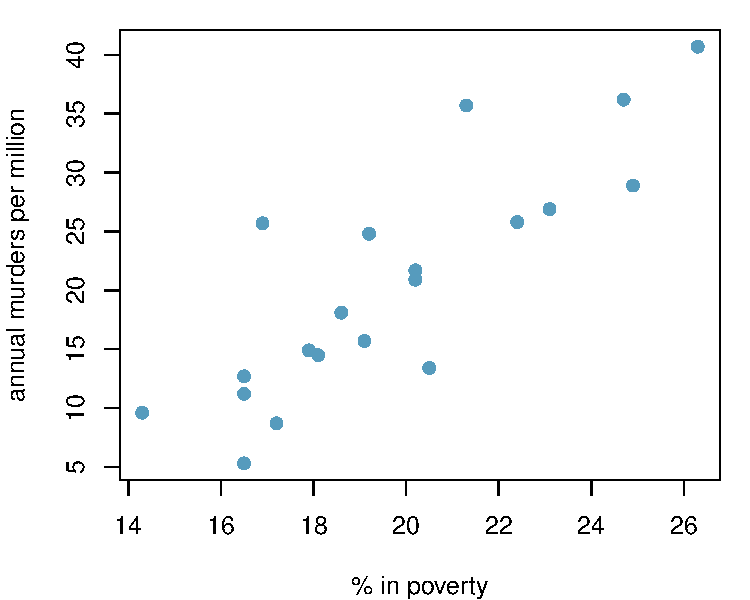
\includegraphics[width=0.9\textwidth]{figures/murder/annual_murders_per_mil_perc_pov}
\end{center}
}

\end{frame}

%%%%%%%%%%%%%%%%%%%%%%%%%%%%%%%%%%%%

\begin{frame}
\frametitle{A note about the intercept}

Sometimes the intercept might be an extrapolation: useful for adjusting the height of the line, but meaningless in the context of the data.

\begin{center}
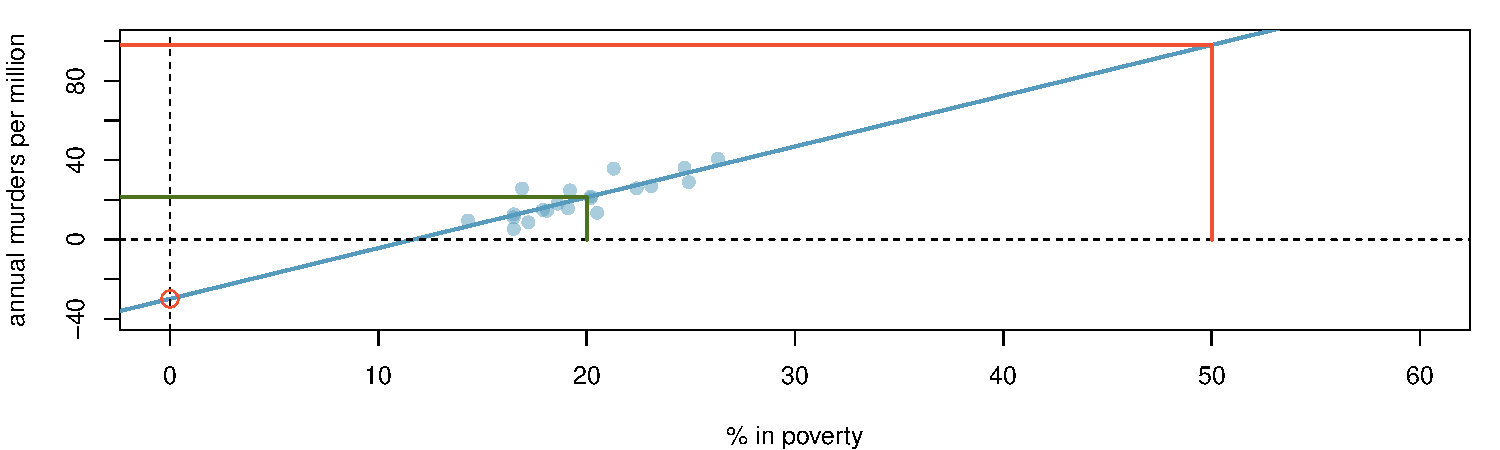
\includegraphics[width=\textwidth]{figures/murder/annual_murders_per_mil_perc_pov_wide}
\end{center}

\end{frame}

%%%%%%%%%%%%%%%%%%%%%%%%%%%%%%%%%%%%

\begin{frame}[fragile]
\frametitle{Calculating predicted values}

\hl{By hand:} $\widehat{murder} = -29.91 + 2.56~poverty$

The predicted number of murders per million per year for a county with 20\% poverty rate is: 

\pause

\[ \widehat{murder} = -29.91 + 2.56 \times 20 = 21.29 \]

\vfill

\pause

\hl{In R:}

{\scriptsize
\begin{Verbatim}[frame=single, formatcom=\color{blue}]
# load data
murder <- read.csv("https://stat.duke.edu/~mc301/data/murder.csv")
# fit model
m_mur_pov <- lm(annual_murders_per_mil ~ perc_pov, data = murder)
# create new data
newdata <- data.frame(perc_pov = 20)
# predict
predict(m_mur_pov, newdata)
\end{Verbatim}
}

\pause

{\scriptsize
\begin{Verbatim}[frame=single, formatcom=\color{gray}]
       1 
21.28663 
\end{Verbatim}
}

\end{frame}

%%%%%%%%%%%%%%%%%%%%%%%%%%%%%%%%%%%%

\subsection{Predicted values also have uncertainty around them}
\label{mi2}

%%%%%%%%%%%%%%%%%%%%%%%%%%%%%%%%%%%%

\begin{frame}
\frametitle{Uncertainty of predictions}

\begin{itemize}

\item Regression models are useful for making predictions for new observations not include in the original dataset.

\pause

\item If the model is good, the predictions should be close to the true value of the response variable for this observation, 
however it may not be exact, i.e. $\hat{y}$ might be different than $y$.

\pause

\item With any prediction we can (and should) also report a measure of uncertainty of the prediction.

\end{itemize}

\end{frame}

%%%%%%%%%%%%%%%%%%%%%%%%%%%%%%%%%%%%

\begin{frame}
\frametitle{Prediction intervals for specific predicted values}

A \hl{prediction interval} for $y$ for a given $x^\star$ is
\[ \hat{y} \pm t^\star_{n - 2} s \sqrt{ 1 + \frac{1}{n} + \frac{(x^\star - \bar{x})^2}{(n - 1)s_x^2} } \]
where $s$ is the standard deviation of the residuals, and $x^\star$ is a new observation.

\pause

\begin{itemize}

\item Interpretation: We are XX\% confident that $\hat{y}$ for given $x^\star$ is within this interval.

\pause

\item The width of the prediction interval for $\hat{y}$ increases as
\begin{itemize}
\item $x^\star$ moves away from the center
\item $s$ (the variability of residuals), i.e. the scatter, increases
\end{itemize}

\pause

\item Prediction level: If we repeat the study of obtaining a regression data set many times, each time forming a XX\% prediction 
interval at $x^\star$, and wait to see what the future value of $y$ is at $x^\star$, then roughly XX\% of the prediction intervals will 
contain the corresponding actual value of $y$.

\end{itemize}

\end{frame}

%%%%%%%%%%%%%%%%%%%%%%%%%%%%%%%%%%%%

\begin{frame}[fragile]
\frametitle{Calculating the prediction interval}

\hl{By hand:}

Don't worry about it...

\pause

$\:$ \\

\hl{In R:}

{\scriptsize
\begin{Verbatim}[frame=single, formatcom=\color{blue}]
# predict
predict(m_mur_pov, newdata, interval = "prediction", level = 0.95)
\end{Verbatim}
}

\pause

{\scriptsize
\begin{Verbatim}[frame=single, formatcom=\color{gray}]
       fit      lwr      upr
1 21.28663 9.418327 33.15493
\end{Verbatim}
}

\pause

We are 95\% confident that the annual murders per million for a county with 20\%
poverty rate is between 9.52 and 33.15.

\end{frame}

%%%%%%%%%%%%%%%%%%%%%%%%%%%%%%%%%%%%


\subsection{$R^2$ assesses model fit -- higher the better}
\label{mi3}

%%%%%%%%%%%%%%%%%%%%%%%%%%%%%%%%%%%%

\begin{frame}[fragile]
\frametitle{(1) $R^2$ assesses model fit -- higher the better}

\begin{itemize}

\item $R^2$: percentage of variability in $y$ explained by the model.

\pause

\item For single predictor regression: $R^2$ is the square of the correlation coefficient, $R$.
{\tiny
\begin{Verbatim}[frame=single, formatcom=\color{blue}]
murder %>%
    summarise(r_sq = cor(annual_murders_per_mil, perc_pov)^2)
\end{Verbatim}
}
{\tiny
\begin{Verbatim}[frame=single, formatcom=\color{gray}]
       r_sq
1 0.7052275
\end{Verbatim}
}

\pause

\item For all regression: $R^2 = \frac{SS_{reg}}{SS_{tot}}$

{\tiny
\begin{Verbatim}[frame=single, formatcom=\color{blue}]
anova(m_mur_pov)
\end{Verbatim}
}

{\tiny
\begin{Verbatim}[frame=single, formatcom=\color{gray}]
Analysis of Variance Table

Response: annual_murders_per_mil
          Df  Sum Sq Mean Sq F value    Pr(>F)    
perc_pov   1 1308.34 1308.34  43.064 3.638e-06 ***
Residuals 18  546.86   30.38  
\end{Verbatim}
}

\end{itemize}

\pause

\begin{adjustwidth}{-0.25cm}{0cm}
{\small
\[ R^2 = \frac{explained~variabilty}{total~variability} \pause =\frac{SS_{reg}}{SS_{tot}} \pause = \frac{1308.34}{1308.34 + 546.86} \pause = \frac{1308.34}{1855.2} \approx 0.71 \]
}
\end{adjustwidth}

\end{frame}

%%%%%%%%%%%%%%%%%%%%%%%%%%%%%%%%%%%%

\begin{frame}
\frametitle{}

\twocol{0.65}{0.35}{
\clicker{$R^2$ for the regression model for predicting annual murders per million based on percentage living in poverty is roughly 
71\%. Which of the following is the correct interpretation of this value?}
}
{
\begin{center}
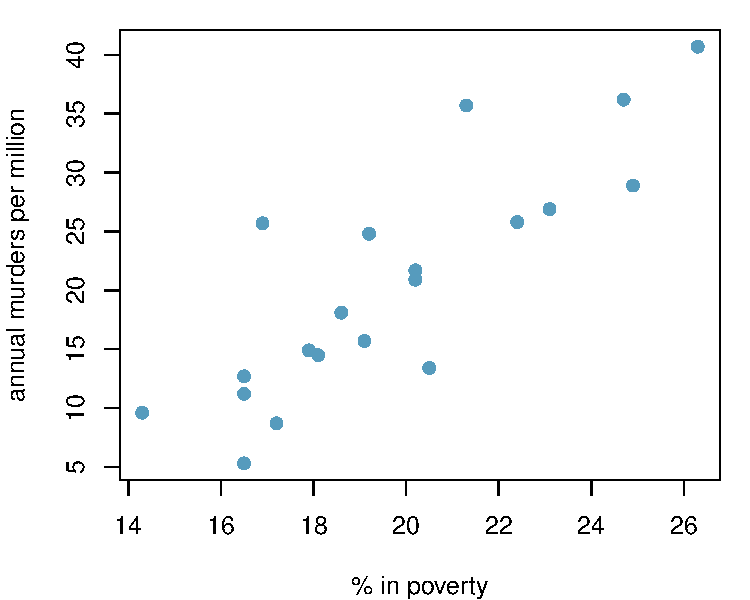
\includegraphics[width=\textwidth]{figures/murder/annual_murders_per_mil_perc_pov}
\end{center}
}

$\:$ \\

\begin{enumerate}[(a)]

\item 71\% of the variability in percentage living in poverty is explained by the model.

\item 84\% of the variability in the murder rates is explained by the model, i.e. percentage living in poverty.

\item \solnMult{71\% of the variability in the murder rates is explained by the model, i.e. percentage living in poverty.}

\item 71\% of the time percentage living in poverty predicts murder rates accurately.

\end{enumerate}

\end{frame}

%%%%%%%%%%%%%%%%%%%%%%%%%%%%%%%%%%

\subsection{Inference for regression uses the $t$-distribution}
\label{mi4}

%%%%%%%%%%%%%%%%%%%%%%%%%%%%%%%%%%%%

\begin{frame}[fragile]
\frametitle{Inference for regression uses the $t$-distribution}

\begin{itemize}

\item Use a T distribution for inference on the slope, with degrees of freedom $n - 2$
\begin{itemize}
\item Degrees of freedom for the slope(s) in regression is $df = n - k - 1$ where $k$~is the number of 
slopes being estimated in the model.
\end{itemize}

\pause

\item Hypothesis testing for a slope: $H_0: \beta_1 = 0$; $H_A: \beta_1 \ne 0$ \\
\begin{itemize}
\item $T_{n-2} = \frac{b_1 - 0}{SE_{b_1}}$
\item p-value = P(observing a slope at least as different from 0 as the one observed if in fact there is no 
relationship between $x$ and $y$
\end{itemize}

\pause

\item Confidence intervals for a slope: 
\begin{itemize}
\item $b_1 \pm T^\star_{n-2} SE_{b_1}$
\item In R:
\end{itemize}

\end{itemize}

{\scriptsize
\begin{Verbatim}[frame=single, formatcom=\color{blue}]
confint(m_mur_pov, level = 0.95)
\end{Verbatim}
}

{\scriptsize
\begin{Verbatim}[frame=single, formatcom=\color{gray}]
                 2.5 %     97.5 %
(Intercept) -46.265631 -13.536694
perc_pov      1.740003   3.378776
\end{Verbatim}
}

\end{frame}

%%%%%%%%%%%%%%%%%%%%%%%%%%%%%%%%%%%%

\subsection{Conditions for regression}
\label{mi5}

%%%%%%%%%%%%%%%%%%%%%%%%%%%%%%%%%%%%

\begin{frame}
\frametitle{Conditions for regression}

\hl{Important regardless of doing inference}

\begin{itemize}

\item Linearity $\rightarrow$ randomly scattered residuals around 0 in the residuals plot -- important regardless of doing inference

\end{itemize}

\pause

$\:$ \\

\hl{Important for inference}

\begin{itemize}

\item Nearly normally distributed residuals $\rightarrow$ histogram or normal probability plot of residuals

\pause

\item Constant variability of residuals (\hl{homoscedasticity}) $\rightarrow$ no fan shape in the residuals plot

\pause

\item Independence of residuals (and hence observations) $\rightarrow$ depends on data collection method, often violated for time-series data

\end{itemize}

\end{frame}

%%%%%%%%%%%%%%%%%%%%%%%%%%%%%%%%%%%%

\begin{frame}
\frametitle{Checking conditions}

\twocol{0.5}{0.5}
{
\clicker{What condition is this linear model obviously and definitely violating?}
\begin{enumerate}[(a)]
\item Linear relationship
\item Non-normal residuals
\item \solnMult{Constant variability}
\item Independence of observations
\end{enumerate}
}
{
\begin{center}
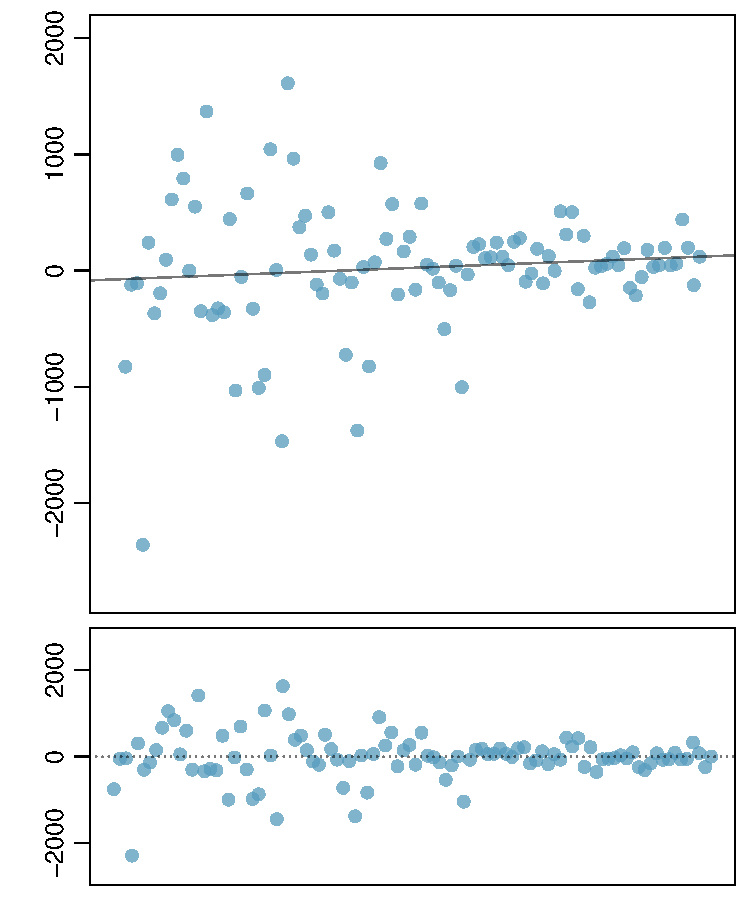
\includegraphics[width=\textwidth]{figures/problems/heteroscedastic}
\end{center}
}

\end{frame}

%%%%%%%%%%%%%%%%%%%%%%%%%%%%%%%%%%%

\begin{frame}
\frametitle{Checking conditions}

\twocol{0.5}{0.5}
{
\clicker{What condition is this linear model obviously and definitely violating?}
\begin{enumerate}[(a)]
\item \solnMult{Linear relationship}
\item Non-normal residuals
\item Constant variability
\item Independence of observations
\end{enumerate}
}
{
\begin{center}
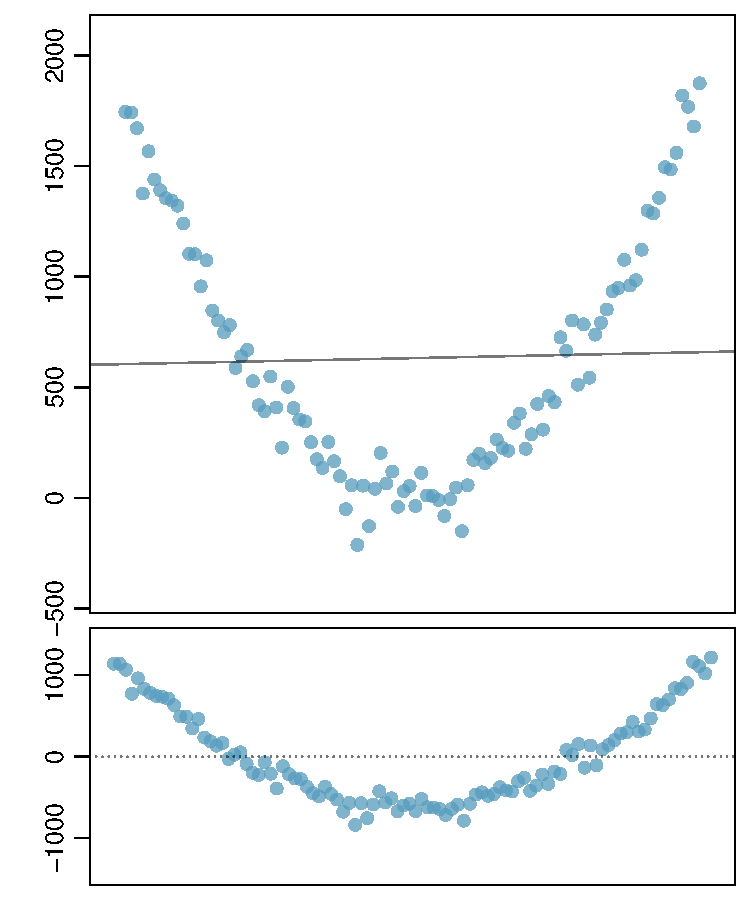
\includegraphics[width=\textwidth]{figures/problems/nonlinear}
\end{center}
}

\end{frame}

%%%%%%%%%%%%%%%%%%%%%%%%%%%%%%%%%%%

\subsection{Type of outlier determines how it should be handled}
\label{mi6}

%%%%%%%%%%%%%%%%%%%%%%%%%%%%%%%%%%%%

\begin{frame}
\frametitle{Type of outlier determines how it should be handled}

\twocol{0.55}{0.5}{
\begin{itemize}
\item \pink{Leverage} point is away from the cloud of points horizontally, does not necessarily change the slope
\item \green{Influential} point changes the \underline{slope} (most likely also has high leverage) -- run the regression with and without that point to determine
\end{itemize}
}
{
\begin{center}
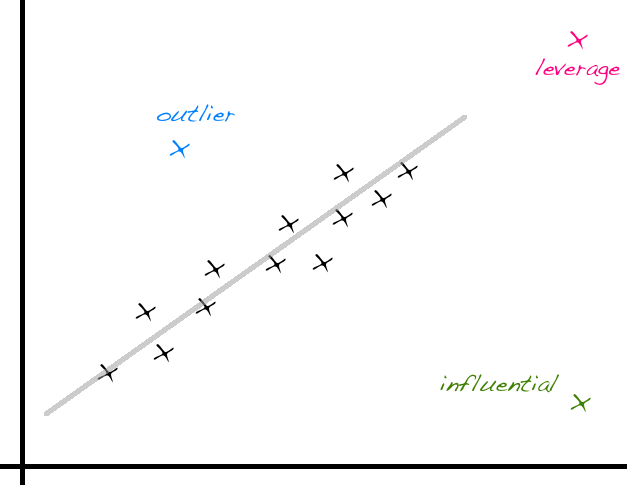
\includegraphics[width=\textwidth]{figures/outlier_sketch}
\end{center}
}

\pause

\begin{adjustwidth}{-0.25cm}{0cm}

\begin{itemize}
\item  \hl{Outlier} is an unusual point without these special characteristics (this one likely affects the intercept only)
\item If clusters (groups of points) are apparent in the data, it might be worthwhile to model the groups separately.
\end{itemize}

\end{adjustwidth}

\end{frame}

%%%%%%%%%%%%%%%%%%%%%%%%%%%%%%%%%%%%

\begin{frame}
\frametitle{}

\vfill

\app{6.2 Linear regression}{See course website for details}

\vfill

\end{frame}

%%%%%%%%%%%%%%%%%%%%%%%%%%%%%%%%%%%

\section{Summary}

%%%%%%%%%%%%%%%%%%%%%%%%%%%%%%%%%%%

\begin{frame}
\frametitle{Summary of main ideas}

\vfill

\begin{enumerate}

\item \nameref{mi1}

\item \nameref{mi2}

\item \nameref{mi3}

\item \nameref{mi4}

\item \nameref{mi5}

\item \nameref{mi6}

\end{enumerate}

\vfill

\end{frame}

%%%%%%%%%%%%%%%%%%%%%%%%%%%%%%%%%%

\end{document}